\documentclass[../main.tex]{subfiles}

\begin{document}
    Różne standardy (czyli \textbf{brak standardu}):
    \begin{itemize}
        \item \textbf{CommonJS} - serwery, Node
        \item \textbf{AMD} (Asynchronous Module Defintion) - przeglądarki
        \item \textbf{ES2015} - wbudowane w język, ale jeszcze niezbyt rozpowszechnione
    \end{itemize}

    \textbf{Moduły} umożliwiają
    \begin{itemize}
        \item \textbf{podział kodu} na (bardziej) \textbf{niezależne} części
        \item łatwiejsze \textbf{współdzielenie} i \textbf{powtórne wykorzystanie} kodu
        \item \textbf{ukrycie implmentacji} i udostęnienie jedynie wybranych funkcji i zmiennych (interfejs)
        \item unikanie \textbf{konfliktów nazw}
    \end{itemize}

    \subsection{CommonJS}
    \begin{itemize}
        \item Plik modułu \textbf{eksportuje} funkcje i obiekty poprzez przypisując je do obiektu \textbf{module.exports}.
        \item Plik wykorzystujący moduł \textbf{ładuje} go przy pomocy funkcji \textbf{require()}.
    \end{itemize}

    \subsection{Express.JS}
    \begin{itemize}
        \item Najpopularniejszy \textbf{framework} w Node
        \item Unopinionated - \textbf{nie narzuca rozwiązań} i struktury. Daje możliwość wyboru.
        \item Podpinanie obsługi pod \textbf{różne metody HTTP} i adresy (routing)
        \item Integracja z \textbf{różnymi silnikami szablonów} stron WWW
        \item Możliwość \textbf{rozszerzania funkcjonalności} za pomocą \textbf{middleware}: obsługa sesji, cookies, logowania użytkowników, itp.
    \end{itemize}

    \subsubsection{Routing}
    \begin{itemize}
        \item Definiowanie obsługi \textbf{poszczególnych metod i ścieżek}: app.get(), .post(), .put(), .delete() itp.
        \item Definiowanie obsługi dla \textbf{dowolnej metody}: app.\textbf{all}().
    \end{itemize}

    \textbf{Express.Router} daje możliwość \textbf{podzielenia obsługi} serwisu/aplikacji webowej na części \textbf{w
    zależności od prefiksu} użytej ścieżki. Można \textbf{delegować} tę obsługe do \textbf{dodatkowego modułu}. Routingi
    zdefinowane w express\_router.js będą dostępne w pod adresem $/express\_router$ oraz $/express\_router/about$.

    \textbf{Ścieżki} używane przy routingu mogą być definiowane jako napisy z \textbf{wzorcami}, np:
    \begin{itemize}
        \item app.get('/ab?cd', callback) - '/abcd' lub '/acd'
        \item app.get('/ab+cd', callback) - '/abcd', '/abbcd', '/abbbcd', \dots
        \item app.get('/ab*cd', callback) - '/abcd', '/abXcd', , '/abDowolnyTekstcd'
        \item app.get(/.*info\$/, callback) - wyrażenia regularne javascript
    \end{itemize}

    \subsubsection{Model MVC (Model-View-Controller)}
    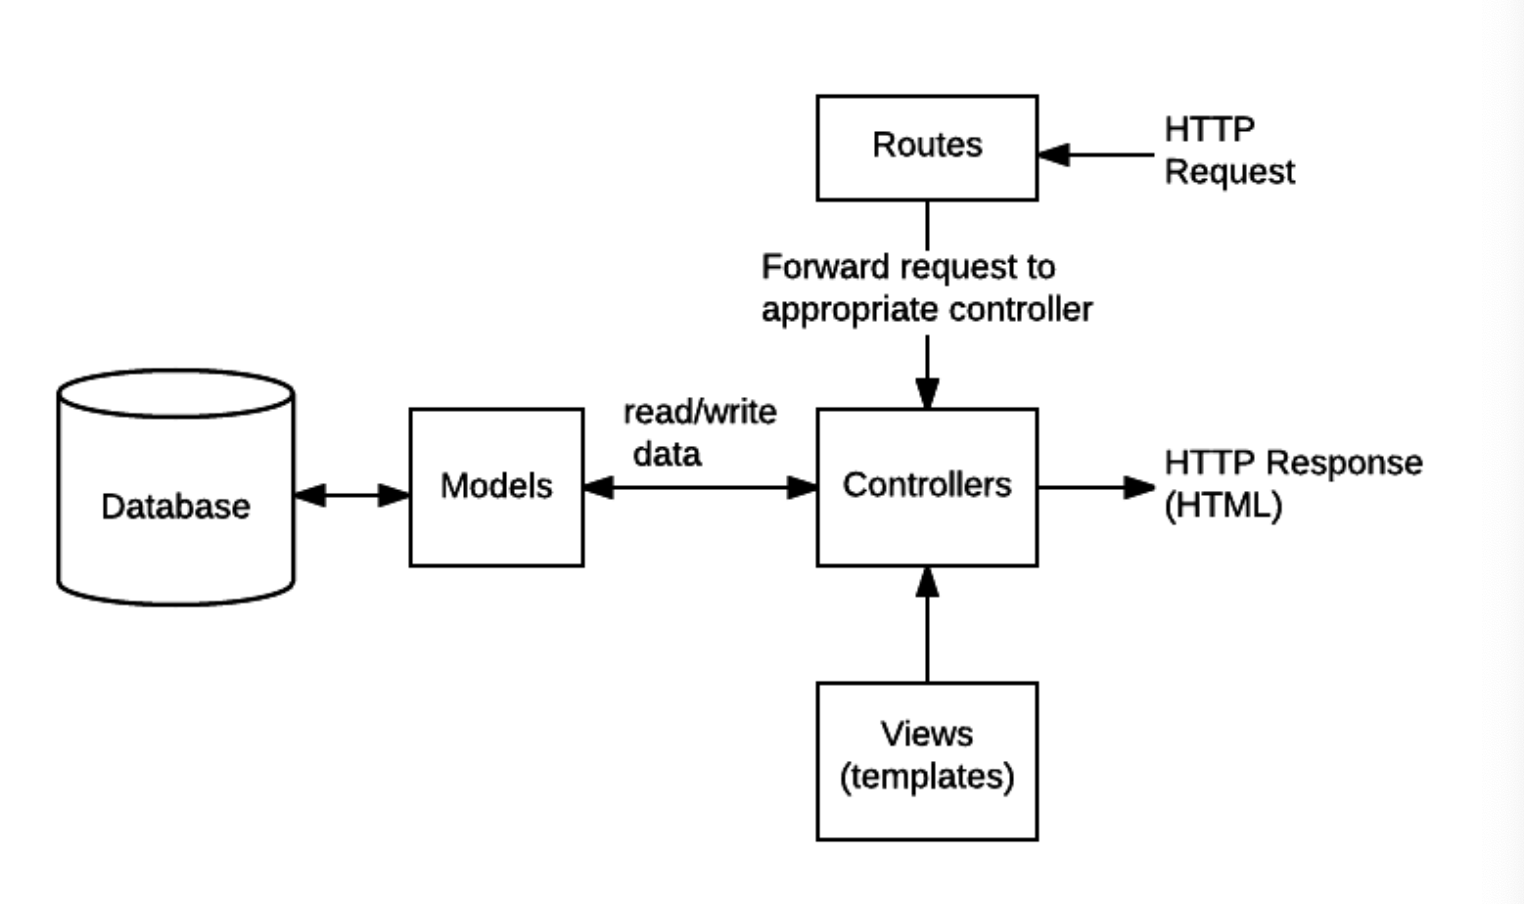
\includegraphics[width=\linewidth]{mvc.png}

    \subsubsection{Szablony}
    Express może współpracować z \textbf{różnymi systemami szablonów} HTML, m.in. Pug, Mustache, EJS.

    \textbf{Pug}
    \begin{itemize}
        \item Zawieranie się elementów jest odzwierciedlone przy pomocy \textbf{wcięć}.
        \item Każda (prawie) linia zaczyna się od \textbf{nazwy znacznika} HTML
        \item Jeśli tag kończy się znakiem \textbf{=}, to dalsza częśc jest traktowana jako \textbf{wyrażenie Javascript}, którego wartość jest wstawiana jako zawartość generowanego elementu.
        \item Można używać \textbf{instrukcji warunkowych} i \textbf{pętli}
        \item Można również \textbf{dziedziczyć/rozszerzać szablony}: polecenia extend i block.
        \item Wygląda jak bardzo uproszczony html, \textbf{bez nawiasów ostrych} <>.
    \end{itemize}


\end{document}